\documentclass[11pt,aspectratio=169]{beamer}
%\documentclass[11pt,aspectratio=169,handout]{beamer}

\usetheme{Boadilla}
\usepackage[utf8]{inputenc}
\usepackage[T1]{fontenc}
\usepackage{lmodern}
\usepackage{lipsum}
\usetheme{default}
\usepackage{listings}
\lstset{language=[90]Fortran,
	basicstyle=\small\ttfamily,
	showtabs=false,
	tabsize=2,      
	keywordstyle=\color{red},
	commentstyle=\color{green},
	morecomment=[l]{!\ }% Comment only with space after !
}


\begin{document}
\author{Zejian Li \\(li.zejian@ictp.it)}
\title{Lecture 2: Numerical Integration (II)}
\subtitle{(Adapted from slides by Gerald Fux)}
%\logo{}
%\institute{}
\date{18. Oct. 2024}
%\subject{}
%\setbeamercovered{transparent}
%\setbeamertemplate{navigation symbols}{}


% ----------------------------------------------------------------
\begin{frame}[plain]
	\maketitle
\end{frame}


% ----------------------------------------------------------------
\section{Introduction}

\begin{frame}
\frametitle{Last Lecture: Left Riemann Sum}
\begin{figure}
	\centering
	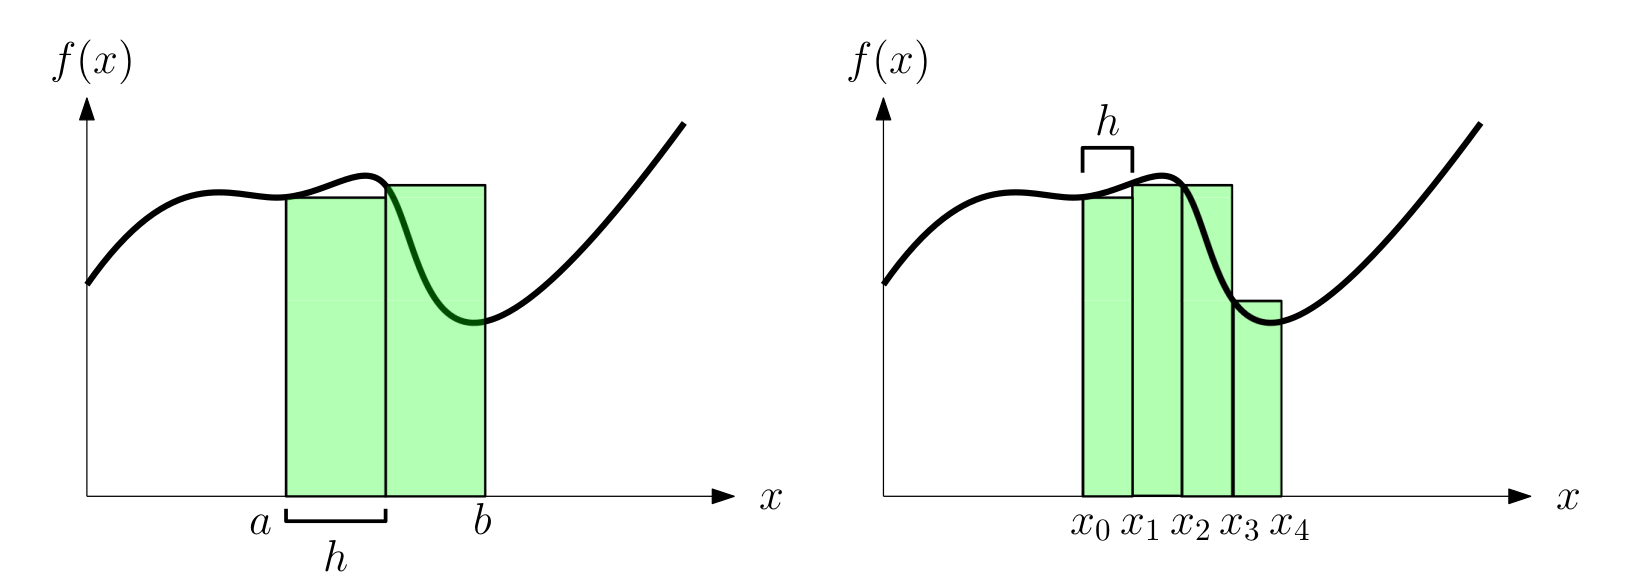
\includegraphics[width=0.6\textwidth]{fig/integration-definition}
\end{figure}
\pause
\begin{equation*}
	I_L(N) \equiv  \sum_{k=0}^{N-1} f(x_k) \cdot h  \quad \text{with} \quad
	\begin{cases}
		h \equiv \frac{b-a}{N} \\
		x_k \equiv a + k \cdot h \\
		k = 0, \ldots, N-1
	\end{cases}
\end{equation*}
\pause
Convergence:
\begin{equation*}
	\int_a^b f(x) \, \mathrm{d}x = I_L(N) + \mathcal{O}\left(\frac{1}{N}\right)
\end{equation*}
\end{frame}

\begin{frame}
\frametitle{Improved Method (a): Midpoint Method}
\begin{figure}
	\centering
	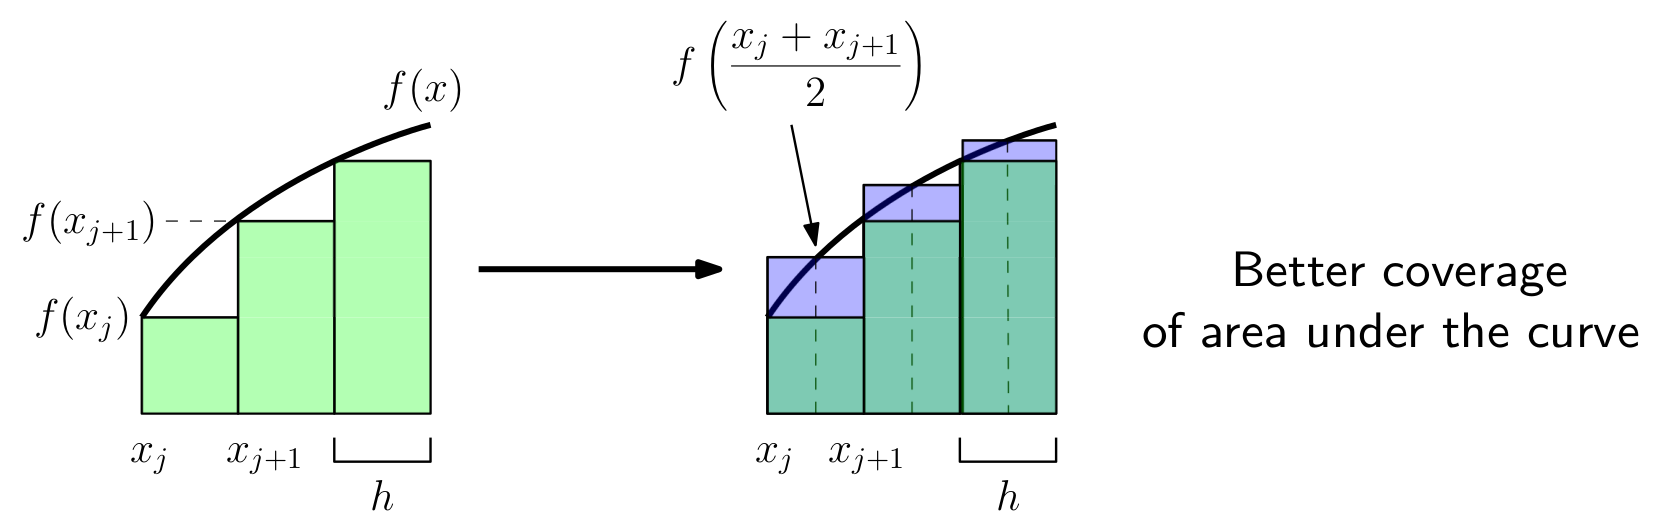
\includegraphics[width=0.8\textwidth]{fig/integration-midpoint-with-text}
\end{figure}
\pause
\begin{equation*}
	I_M(N) \equiv  \sum_{k=0}^{N-1} f\left(\frac{x_k+x_{k+1}}{2}\right) \cdot h  \quad \text{with} \quad
	\begin{cases}
		h \equiv \frac{b-a}{N} \\
		x_k \equiv a + k \cdot h \\
		k = 0, \ldots, N-1
	\end{cases}
\end{equation*}

\only<3|handout:0>{
	Better convergence:
	\begin{equation*}
		\int_a^b f(x) \, \mathrm{d}x = I_M(N) + \mathcal{O}\left(\frac{1}{N^2}\right)
	\end{equation*}
}

\onslide<4>{
	Better convergence:
	\begin{equation*}
		\int_a^b f(x) \, \mathrm{d}x = I_M(N) + \mathcal{O}\left(\frac{1}{N^2}\right) =  I_M(h) + \mathcal{O}\left(h^2\right)
	\end{equation*}
}
\end{frame}

\begin{frame}
	\frametitle{Improved Method (b): Trapezoidal Method}
\begin{figure}
	\centering
	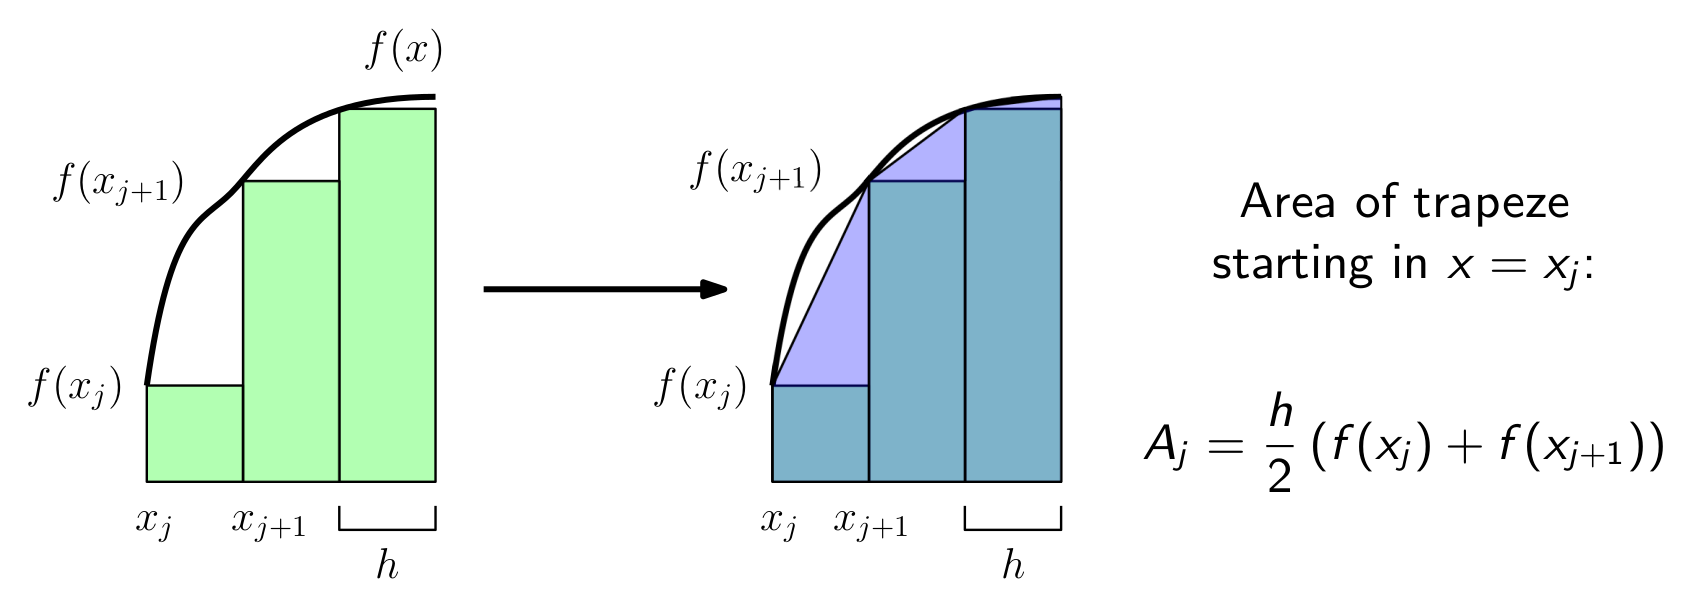
\includegraphics[width=0.7\textwidth]{fig/integration-trapez-with-text}
\end{figure}
\pause
\begin{equation*}
	I_T(N) \equiv  \sum_{k=0}^{N-1} \left[ f(x_k)+f(x_{k+1}) \right] \cdot \frac{h}{2}  \quad \text{with} \quad
	\begin{cases}
		h \equiv \frac{b-a}{N} \\
		x_k \equiv a + k \cdot h \\
		k = 0, \ldots, N
	\end{cases}
\end{equation*}

\pause

Convergence (same as the midpoint method):
\begin{equation*}
	\int_a^b f(x) \, \mathrm{d}x = I_T(h) + \mathcal{O}\left(h^2\right)
\end{equation*}

\end{frame}


\begin{frame}
\frametitle{Improved Method (b): Trapezoidal Method}
\begin{align*}
	I_T(N) & \equiv  \sum_{k=0}^{N-1} \left[ f(x_k)+f(x_{k+1}) \right] \cdot \frac{h}{2} \\
	 & \equiv \frac{h}{2}\left[\underbrace{f(x_0) + f(x_1)} + \underbrace{f(x_1) + f(x_2)} + \underbrace{f(x_2) + f(x_3)} + \ldots \right]
\end{align*}
\begin{block}{(Better) reformulation of the trapezoidal method}
	Note that $f(x_1), f(x_2), \ldots, f(x_{N-2})$ each appear twice in the sum. Because it might be very hard to evaluate $f(x)$  it is better to \textbf{calculate each $f(x_j)$ only once instead of twice}. We thus implement the method in the rewritten form $\ldots$
	\begin{equation*}
		I_T(N) = \frac{h}{2} \left[ f(x_0) + \left(\sum_{k=1}^{N-1}  2f(x_k)\right)+f(x_{N}) \right] \mathrm{.}
	\end{equation*}
\end{block}

\end{frame}

\begin{frame}
\frametitle{Improved Method (c): Simpson Method}
Next improvement: from Trapeziods $\rightarrow$ to \textbf{parabolic arcs.}
\pause
\begin{figure}
	\centering
	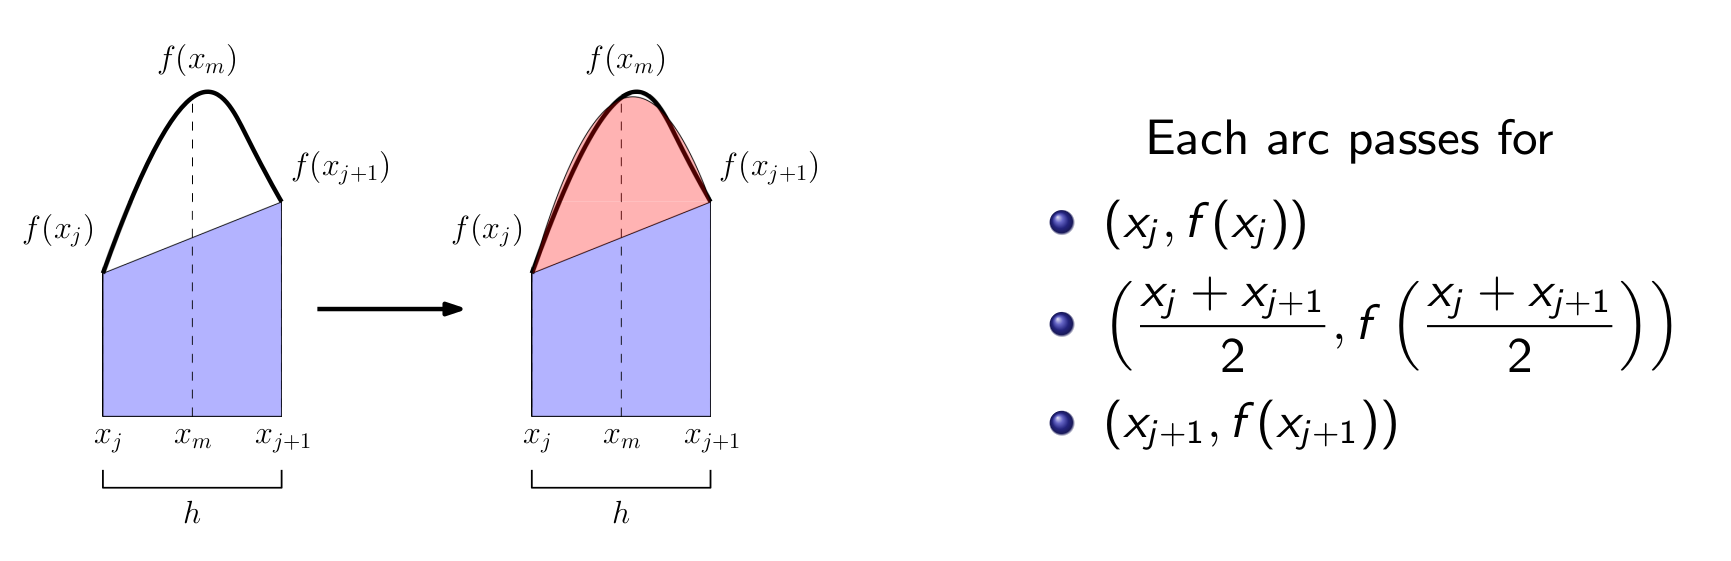
\includegraphics[width=0.7\textwidth]{fig/integration-simpson-with-text}
\end{figure}%
\pause
\begin{equation*}
\text{Algebra yields that the area is:} \quad A_j = \frac{h}{6} \left[ f(x_j) + 4 f\left(\frac{x_j + x_{j+1}}{2}\right) + f(x_{j+1}) \right]
\end{equation*}

\pause
\begin{equation*}
	I_S(N) \equiv \frac{h}{6} \left[ f(x_0) + 2\sum_{k=1}^{N-1} f(x_k)+4\sum_{k=0}^{N-1}f\left(\frac{x_k + x_{k+1}}{2}\right) + f(x_{N}) \right] 
	\quad \text{with} \quad
	\begin{cases}
		h \equiv \frac{b-a}{N} \\
		x_k \equiv a + k \cdot h \\
		k = 0, \ldots, N
	\end{cases}
\end{equation*}

\end{frame}

\begin{frame}
\frametitle{Improved Method (c): Simpson Method}
\begin{figure}
	\centering
	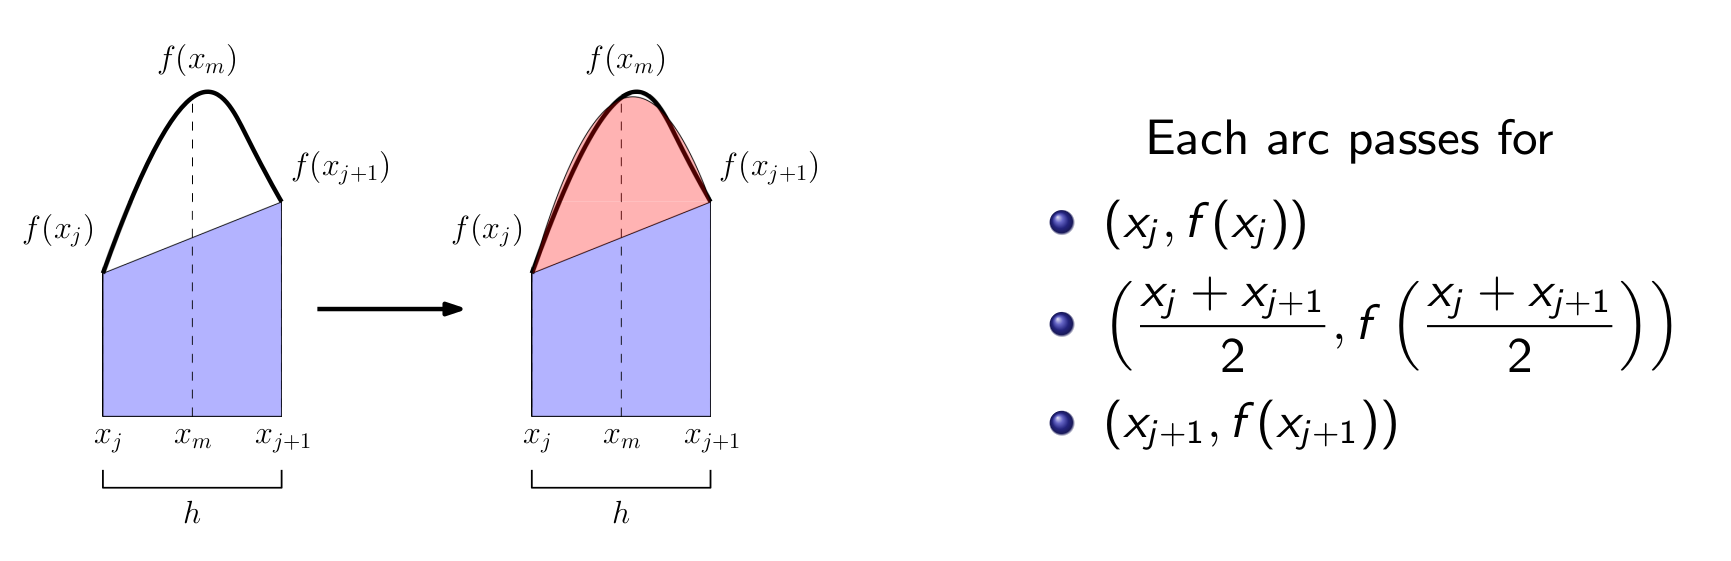
\includegraphics[width=0.7\textwidth]{fig/integration-simpson-with-text}
\end{figure}%
\begin{equation*}
	I_S(N) \equiv \frac{h}{6} \left[ f(x_0) + 2\sum_{k=1}^{N-1} f(x_k)+4\sum_{k=0}^{N-1}f\left(\frac{x_k + x_{k+1}}{2}\right) + f(x_{N}) \right] 
	\quad \text{with} \quad
	\begin{cases}
		h \equiv \frac{b-a}{N} \\
		x_k \equiv a + k \cdot h \\
		k = 0, \ldots, N
	\end{cases}
\end{equation*}

Convergence:
\begin{equation*}
	\int_a^b f(x) \, \mathrm{d}x = I_S(h) + \mathcal{O}\left(h^4\right)
\end{equation*}
	
\end{frame}

\begin{frame}
\frametitle{Advanced Integration Methods}
Beyond these basic approaches many advanced / specialized methods exist. E.g.:
\pause
\begin{columns}
	\column{0.6\textwidth}
	\textbf{Adaptive integration}: \\
	Make the grid finer where the function changes faster.
	\column{0.4\textwidth}
	\begin{figure}
		\centering
		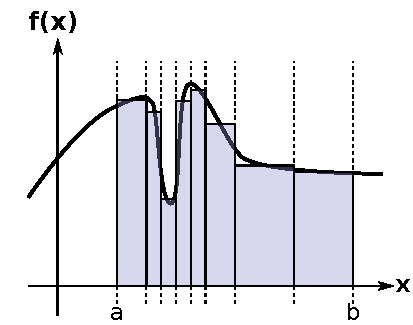
\includegraphics[width=0.4\textwidth]{fig/integration-adaptive}
	\end{figure}%
\end{columns}

\pause
\begin{columns}
	\column{0.6\textwidth}
	\textbf{Gaussian quadratures}: \\
	Mathematically optimal grid.
	\column{0.4\textwidth}
	\begin{figure}
		\centering
		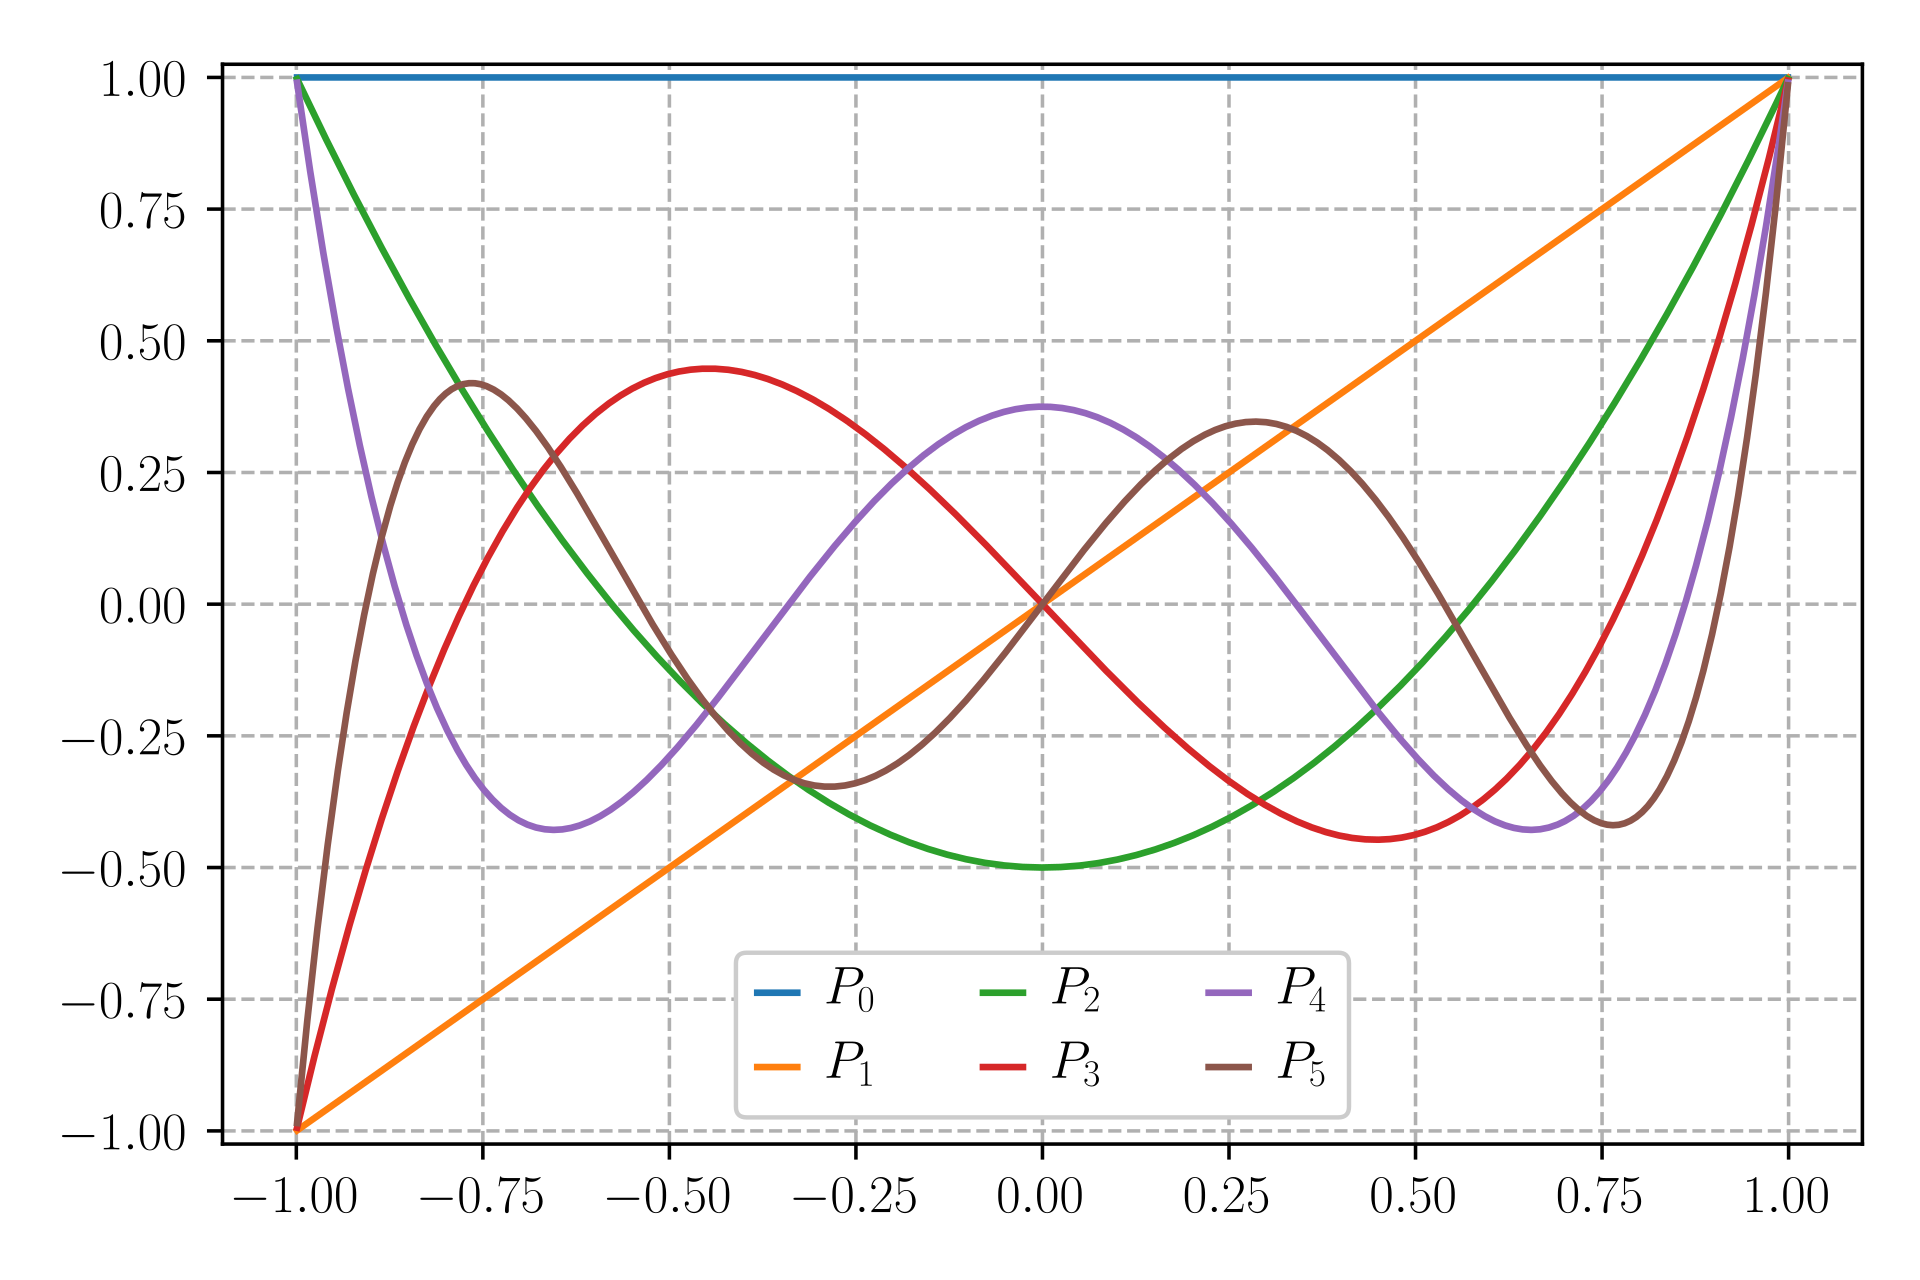
\includegraphics[width=0.4\textwidth]{fig/integration-legendre}
	\end{figure}%
\end{columns}

\pause
\begin{columns}
	\column{0.6\textwidth}
	\textbf{Monte Carlo integration}: \\
	Use a randomized grid; best in high dimensions.
	\column{0.4\textwidth}
	\begin{figure}
		\centering
		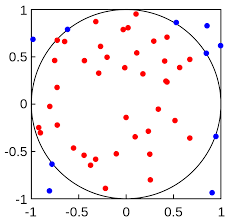
\includegraphics[width=0.3\textwidth]{fig/integration-monte-carlo}
	\end{figure}%
\end{columns}

\end{frame}

\begin{frame}
\frametitle{Assignment 10}
Write a FORTRAN program that computes $\int_a^b f(x)\, \mathrm{d}x$ for  $f(x) = \dfrac{16x-16}{x^4 - 2x^3+4x-4}$ using the Midpoint, Trapeze, and Simpson method:
\begin{itemize}
\item Write a function (for each of the three methods) that takes the bounds $a$ and $b$, and the desired precision $\epsilon$.
\pause
\item The function should integrate with the Midpoint/Trapeze/Simpson method, increasing N until the precision is achieved.
\pause
\item The function should print the result at each step together with the current value for $N$ (this is just for us to see what is happening during the calculation).
\pause
\item Test the function by calculating $\int_0^1 f(x)\, \mathrm{d}x$ with error threshold $10^{-5}$ in the main program and print the result.
\pause
\item Submit your code as \texttt{Ass10.YourLastName.f90} to \texttt{li.zejian@ictp.it} before the next lesson.
\end{itemize}
\textbf{Bonus question:}
\begin{itemize}
\item Comment (in the email) about how often the function f(x) is called in total for each method. Which method is the most efficient?
\end{itemize}
\end{frame}

\end{document}